\documentclass[tikz,border=0pt]{standalone}
%\usepackage{mathptmx}
\usepackage[utf8]{inputenc}
\usetikzlibrary{patterns,decorations.pathmorphing,positioning,arrows,automata}

\begin{document}
	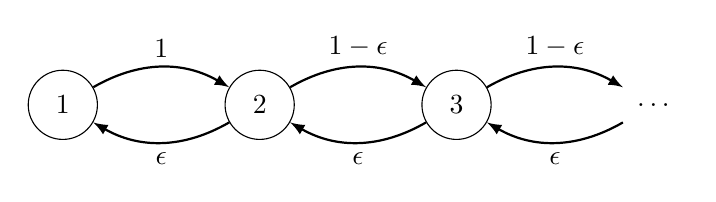
\begin{tikzpicture}[node distance=2.5cm,->,>=latex,auto,
		every edge/.append style={thick}
		]
		\node[state] (1) {$1$};
		\node[state] (2) [right of=1] {$2$};  
		\node[state] (3) [right of=2] {$3$};  
		\node[state, draw=none] (4) [right of=3] {$\dots$};  
		
		\path (1) edge[bend left] node{$1$} (2);
		\path (2) edge[bend left] node{$\epsilon$} (1);
		\path (2) edge[bend left] node{$1-\epsilon$} (3);
		\path (3) edge[bend left] node{$\epsilon$} (2);
		\path (3) edge[bend left] node{$1-\epsilon$} (4);
		\path (4) edge[bend left] node{$\epsilon$} (3);
	\end{tikzpicture}
\end{document}